%================================================
%    位相空間まとめノート
%================================================

% -----------------------
% preamble
% -----------------------
% ここから本文 (\begin{document}) までの
% ソースコードに変更を加えた場合は
% 編集者まで連絡してください. 
% Don't change preamble code yourself. 
% If you add something
% (usepackage, newtheorem, newcommand, renewcommand),
% please tell it 
% to the editor of institutional paper of RUMS.

% ------------------------
% documentclass
% ------------------------
\documentclass[11pt, a4paper, dvipdfmx]{jsarticle}

% ------------------------
% usepackage
% ------------------------
\usepackage{algorithm}
\usepackage{algorithmic}
\usepackage{amscd}
\usepackage{amsfonts}
\usepackage{amsmath}
\usepackage[psamsfonts]{amssymb}
\usepackage{amsthm}
\usepackage{ascmac}
\usepackage{bm}
\usepackage{color}
\usepackage{enumerate}
\usepackage{fancybox}
\usepackage[stable]{footmisc}
\usepackage{graphicx}
\usepackage{listings}
\usepackage{mathrsfs}
\usepackage{mathtools}
\usepackage{otf}
\usepackage{pifont}
\usepackage{proof}
\usepackage{subfigure}
\usepackage{tikz}
\usepackage{verbatim}
\usepackage[all]{xy}
\usepackage{url}
\usetikzlibrary{cd}



% ================================
% パッケージを追加する場合のスペース 
%\usepackage{calligra}
\usepackage[dvipdfmx]{hyperref}
\usepackage{xcolor}
\definecolor{darkgreen}{rgb}{0,0.45,0} 
\definecolor{darkred}{rgb}{0.75,0,0}
\definecolor{darkblue}{rgb}{0,0,0.6} 
\hypersetup{
    colorlinks=true,
    citecolor=darkgreen,
    linkcolor=darkred,
    urlcolor=darkblue,
}
\usepackage{pxjahyper}
\usepackage{layout}
%=================================


% --------------------------
% theoremstyle
% --------------------------
\theoremstyle{definition}

% --------------------------
% newtheoem
% --------------------------

% 日本語で定理, 命題, 証明などを番号付きで用いるためのコマンドです. 
% If you want to use theorem environment in Japanece, 
% you can use these code. 
% Attention!
% All theorem enivironment numbers depend on 
% only section numbers.
\newtheorem{Axiom}{公理}[section]
\newtheorem{Definition}[Axiom]{定義}
\newtheorem{Theorem}[Axiom]{定理}
\newtheorem{Proposition}[Axiom]{命題}
\newtheorem{Lemma}[Axiom]{補題}
\newtheorem{Corollary}[Axiom]{系}
\newtheorem{Example}[Axiom]{例}
\newtheorem{Claim}[Axiom]{主張}
\newtheorem{Property}[Axiom]{性質}
\newtheorem{Attention}[Axiom]{注意}
\newtheorem{Question}[Axiom]{問}
\newtheorem{Problem}[Axiom]{問題}
\newtheorem{Consideration}[Axiom]{考察}
\newtheorem{Alert}[Axiom]{警告}
\newtheorem{Fact}[Axiom]{事実}
\newtheorem{com}[Axiom]{コメント}


% 日本語で定理, 命題, 証明などを番号なしで用いるためのコマンドです. 
% If you want to use theorem environment with no number in Japanese, You can use these code.
\newtheorem*{Axiom*}{公理}
\newtheorem*{Definition*}{定義}
\newtheorem*{Theorem*}{定理}
\newtheorem*{Proposition*}{命題}
\newtheorem*{Lemma*}{補題}
\newtheorem*{Example*}{例}
\newtheorem*{Corollary*}{系}
\newtheorem*{Claim*}{主張}
\newtheorem*{Property*}{性質}
\newtheorem*{Attention*}{注意}
\newtheorem*{Question*}{問}
\newtheorem*{Problem*}{問題}
\newtheorem*{Consideration*}{考察}
\newtheorem*{Alert*}{警告}
\newtheorem*{Fact*}{事実}
\newtheorem*{com*}{コメント}



% 英語で定理, 命題, 証明などを番号付きで用いるためのコマンドです. 
% If you want to use theorem environment in English, You can use these code.
%all theorem enivironment number depend on only section number.
\newtheorem{Axiom+}{Axiom}[section]
\newtheorem{Definition+}[Axiom+]{Definition}
\newtheorem{Theorem+}[Axiom+]{Theorem}
\newtheorem{Proposition+}[Axiom+]{Proposition}
\newtheorem{Lemma+}[Axiom+]{Lemma}
\newtheorem{Example+}[Axiom+]{Example}
\newtheorem{Corollary+}[Axiom+]{Corollary}
\newtheorem{Claim+}[Axiom+]{Claim}
\newtheorem{Property+}[Axiom+]{Property}
\newtheorem{Attention+}[Axiom+]{Attention}
\newtheorem{Question+}[Axiom+]{Question}
\newtheorem{Problem+}[Axiom+]{Problem}
\newtheorem{Consideration+}[Axiom+]{Consideration}
\newtheorem{Alert+}{Alert}
\newtheorem{Fact+}[Axiom+]{Fact}
\newtheorem{Remark+}[Axiom+]{Remark}

% ----------------------------
% commmand
% ----------------------------
% 執筆に便利なコマンド集です. 
% コマンドを追加する場合は下のスペースへ. 

% 集合の記号 (黒板文字)
\newcommand{\NN}{\mathbb{N}}
\newcommand{\ZZ}{\mathbb{Z}}
\newcommand{\QQ}{\mathbb{Q}}
\newcommand{\RR}{\mathbb{R}}
\newcommand{\CC}{\mathbb{C}}
\newcommand{\PP}{\mathbb{P}}
\newcommand{\KK}{\mathbb{K}}


% 集合の記号 (太文字)
\newcommand{\nn}{\mathbf{N}}
\newcommand{\zz}{\mathbf{Z}}
\newcommand{\qq}{\mathbf{Q}}
\newcommand{\rr}{\mathbf{R}}
\newcommand{\cc}{\mathbf{C}}
\newcommand{\pp}{\mathbf{P}}
\newcommand{\kk}{\mathbf{K}}

% 特殊な写像の記号
\newcommand{\ev}{\mathop{\mathrm{ev}}\nolimits} % 値写像
\newcommand{\pr}{\mathop{\mathrm{pr}}\nolimits} % 射影
\newcommand{\dist}{\mathop{\mathrm{dist}}\nolimits} % 距離関数


% 偏微分作用素の記号
\newcommand{\p}{\partial}

% 角カッコの記号 (内積は下にマクロがあります)
\newcommand{\lan}{\langle}
\newcommand{\ran}{\rangle}

% 位相空間
\newcommand{\Int}[1][]{\mathop{\mathrm{Int}}\nolimits_{#1}}
\newcommand{\Cl}[1][]{\mathop{\mathrm{Cl}}\nolimits_{#1}}
\newcommand{\Bd}[1][]{\mathop{\mathrm{Bd}}\nolimits_{#1}}
\newcommand{\Fr}[1][]{\mathop{\mathrm{Fr}}\nolimits_{#1}}






\newcommand{\indlim}[1][]{\mathop{\varinjlim}\limits_{#1}}
\newcommand{\sindlim}[1][]{\smash{\mathop{\varinjlim}\limits_{#1}}\,}
\newcommand{\Pro}{\mathrm{Pro}}
\newcommand{\Ind}{\mathrm{Ind}}
\newcommand{\prolim}[1][]{\mathop{\varprojlim}\limits_{#1}}
\newcommand{\sprolim}[1][]{\smash{\mathop{\varprojlim}\limits_{#1}}\,}





% 射の集合など
\newcommand{\Map}{\mathop{\mathrm{Map}}\nolimits}
\newcommand{\Hom}{\mathop{\mathrm{Hom}}\nolimits}
\newcommand{\End}{\mathop{\mathrm{End}}\nolimits}
\newcommand{\Aut}{\mathop{\mathrm{Aut}}\nolimits}
\newcommand{\Mor}{\mathop{\mathrm{Mor}}\nolimits}

% その他便利なコマンド
\newcommand{\dip}{\displaystyle} % 本文中で数式モード
\newcommand{\e}{\varepsilon} % イプシロン
\newcommand{\dl}{\delta} % デルタ
\newcommand{\pphi}{\varphi} % ファイ
\newcommand{\ti}{\tilde} % チルダ
\newcommand{\pal}{\parallel} % 平行
\newcommand{\op}{{\rm op}} % 双対を取る記号
\newcommand{\lcm}{\mathop{\mathrm{lcm}}\nolimits} % 最小公倍数の記号
\newcommand{\Probsp}{(\Omega, \F, \P)} 
\newcommand{\argmax}{\mathop{\rm arg~max}\limits}
\newcommand{\argmin}{\mathop{\rm arg~min}\limits}





% ================================
% コマンドを追加する場合のスペース 
\renewcommand\proofname{\bf 証明} % 証明
\numberwithin{equation}{subsection}
\newcommand{\cTop}{\textsf{Top}}
%\newcommand{\cOpen}{\textsf{Open}}
\newcommand{\Op}{\mathop{\textsf{Open}}\nolimits}
\newcommand{\Ob}{\mathop{\textrm{Ob}}\nolimits}
\newcommand{\id}{\mathop{\mathrm{id}}\nolimits}
\newcommand{\pt}{\mathop{\mathrm{pt}}\nolimits}
\newcommand{\res}{\mathop{\rho}\nolimits}
\newcommand{\Ring}{\mathop{\textsf{Ring}}\nolimits}
\newcommand{\cAb}{\mathop{\textsf{Ab}}\nolimits}
\newcommand{\Sh}{\mathop{\textsf{Sh}}\nolimits}
\newcommand{\PSh}{\mathop{\textsf{PSh}}\nolimits}
\newcommand{\Ker}{\mathop{\mathrm{Ker}}\nolimits}
\newcommand{\im}{\mathop{\mathrm{Im}}\nolimits}
\newcommand{\Coker}{\mathop{\mathrm{Coker}}\nolimits}
\newcommand{\Coim}{\mathop{\mathrm{Coim}}\nolimits}
\newcommand{\Ht}{\mathop{\mathrm{Ht}}\nolimits}
\newcommand{\colim}{\mathop{\mathrm{colim}}}
\newcommand{\ori}{\mathop{\textsf{or}}\nolimits}


\newcommand{\cat}{\mathcal{C}}%一般の圏の記号
\newcommand{\Comp}{\mathop{\mathrm{C}}\nolimits}%複体の圏
\newcommand{\Komp}{\mathop{\mathrm{K}}\nolimits}%複体のホモトピー圏
\newcommand{\CCat}{\Comp(\cat)}%圏Cの複体の圏
\newcommand{\KCat}{\Komp(\cat)}%圏Cの複体のホモトピー圏
\newcommand{\HOM}{\mathop{\mathscr{H}\hspace{-2pt}om}\nolimits}%内部Hom
\newcommand{\RHOM}{\mathop{\mathrm{R}\hspace{-1.5pt}\HOM}\nolimits}
\newcommand{\muS}{\mathop{\mathrm{SS}}\nolimits}
\newcommand{\RG}{\mathop{\mathrm{R}\hspace{-0pt}\Gamma}\nolimits}

\newcommand{\limf}{\mathop{\text{``}\hspace{-0.7pt}\varinjlim\hspace{-1.5pt}\text{''}}}
\newcommand{\sumf}{\mathop{\text{``}\hspace{-0.7pt}\bigoplus\hspace{-1.5pt}\text{''}}}

\newcommand{\hh}{\mathop{\mathrm{h}}\nolimits}



%筆記体
\newcommand{\cA}{\mcal{A}}
\newcommand{\cB}{\mcal{B}}
\newcommand{\cC}{\mcal{C}}
\newcommand{\cD}{\mcal{D}}
\newcommand{\cE}{\mcal{E}}
\newcommand{\cF}{\mcal{F}}
\newcommand{\cG}{\mcal{G}}
\newcommand{\cH}{\mcal{H}}
\newcommand{\cI}{\mcal{I}}
\newcommand{\cJ}{\mcal{J}}
\newcommand{\cK}{\mcal{K}}
\newcommand{\cL}{\mcal{L}}
\newcommand{\cM}{\mcal{M}}
\newcommand{\cN}{\mcal{N}}
\newcommand{\cO}{\mcal{O}}
\newcommand{\cP}{\mcal{P}}
\newcommand{\cQ}{\mcal{Q}}
\newcommand{\cR}{\mcal{R}}
\newcommand{\cS}{\mcal{S}}
\newcommand{\cT}{\mcal{T}}
\newcommand{\cU}{\mcal{U}}
\newcommand{\cV}{\mcal{V}}
\newcommand{\cW}{\mcal{W}}
\newcommand{\cX}{\mcal{X}}
\newcommand{\cY}{\mcal{Y}}
\newcommand{\cZ}{\mcal{Z}}

%スクリプト体
\newcommand{\scA}{\mathscr{A}}
\newcommand{\scB}{\mathscr{B}}
\newcommand{\scC}{\mathscr{C}}
\newcommand{\scD}{\mathscr{D}}
\newcommand{\scE}{\mathscr{E}}
\newcommand{\scF}{\mathscr{F}}
\newcommand{\scG}{\mathscr{G}}
\newcommand{\scH}{\mathscr{H}}
\newcommand{\scI}{\mathscr{I}}
\newcommand{\scJ}{\mathscr{J}}
\newcommand{\scK}{\mathscr{K}}
\newcommand{\scL}{\mathscr{L}}
\newcommand{\scM}{\mathscr{M}}
\newcommand{\scN}{\mathscr{N}}
\newcommand{\scO}{\mathscr{O}}
\newcommand{\scP}{\mathscr{P}}
\newcommand{\scQ}{\mathscr{Q}}
\newcommand{\scR}{\mathscr{R}}
\newcommand{\scS}{\mathscr{S}}
\newcommand{\scT}{\mathscr{T}}
\newcommand{\scU}{\mathscr{U}}
\newcommand{\scV}{\mathscr{V}}
\newcommand{\scW}{\mathscr{W}}
\newcommand{\scX}{\mathscr{X}}
\newcommand{\scY}{\mathscr{Y}}
\newcommand{\scZ}{\mathscr{Z}}


\newcommand{\ibA}{\mathop{\text{\textit{\textbf{A}}}}}
\newcommand{\ibB}{\mathop{\text{\textit{\textbf{B}}}}}
\newcommand{\ibC}{\mathop{\text{\textit{\textbf{C}}}}}
\newcommand{\ibD}{\mathop{\text{\textit{\textbf{D}}}}}
\newcommand{\ibE}{\mathop{\text{\textit{\textbf{E}}}}}
\newcommand{\ibF}{\mathop{\text{\textit{\textbf{F}}}}}
\newcommand{\ibG}{\mathop{\text{\textit{\textbf{G}}}}}
\newcommand{\ibH}{\mathop{\text{\textit{\textbf{H}}}}}
\newcommand{\ibI}{\mathop{\text{\textit{\textbf{I}}}}}
\newcommand{\ibJ}{\mathop{\text{\textit{\textbf{J}}}}}
\newcommand{\ibK}{\mathop{\text{\textit{\textbf{K}}}}}
\newcommand{\ibL}{\mathop{\text{\textit{\textbf{L}}}}}
\newcommand{\ibM}{\mathop{\text{\textit{\textbf{M}}}}}
\newcommand{\ibN}{\mathop{\text{\textit{\textbf{N}}}}}
\newcommand{\ibO}{\mathop{\text{\textit{\textbf{O}}}}}
\newcommand{\ibP}{\mathop{\text{\textit{\textbf{P}}}}}
\newcommand{\ibQ}{\mathop{\text{\textit{\textbf{Q}}}}}
\newcommand{\ibR}{\mathop{\text{\textit{\textbf{R}}}}}
\newcommand{\ibS}{\mathop{\text{\textit{\textbf{S}}}}}
\newcommand{\ibT}{\mathop{\text{\textit{\textbf{T}}}}}
\newcommand{\ibU}{\mathop{\text{\textit{\textbf{U}}}}}
\newcommand{\ibV}{\mathop{\text{\textit{\textbf{V}}}}}
\newcommand{\ibW}{\mathop{\text{\textit{\textbf{W}}}}}
\newcommand{\ibX}{\mathop{\text{\textit{\textbf{X}}}}}
\newcommand{\ibY}{\mathop{\text{\textit{\textbf{Y}}}}}
\newcommand{\ibZ}{\mathop{\text{\textit{\textbf{Z}}}}}

\newcommand{\ibx}{\mathop{\text{\textit{\textbf{x}}}}}


\newcommand{\sm}{\raisebox{2.33pt}{~\rule{6.4pt}{1.3pt}~}}
\newcommand{\smi}{\mathrel{\raisebox{2.33pt}{\rule{6.4pt}{1.3pt}}}}












\usepackage{framed}
\definecolor{lightgray}{rgb}{0.75,0.75,0.75}
\renewenvironment{leftbar}{%
  \def\FrameCommand{\textcolor{lightgray}{\vrule width 4pt} \hspace{10pt}}% 
  \MakeFramed {\advance\hsize-\width \FrameRestore}}%
{\endMakeFramed}
\newenvironment{redleftbar}{%
  \def\FrameCommand{\textcolor{lightgray}{\vrule width 1pt} \hspace{10pt}}% 
  \MakeFramed {\advance\hsize-\width \FrameRestore}}%
 {\endMakeFramed}




% =================================


%================================================
% 自前の定理環境
%   https://mathlandscape.com/latex-amsthm/
% を参考にした
\newtheoremstyle{mystyle}%   % スタイル名
    {5pt}%                   % 上部スペース
    {5pt}%                   % 下部スペース
    {}%              % 本文フォント
    {}%                  % 1行目のインデント量
    {\bfseries}%                      % 見出しフォント
    {.}%                     % 見出し後の句読点
    {12pt}%                     % 見出し後のスペース
    {\thmname{#1}\thmnumber{ #2}\thmnote{{\hspace{2pt}\normalfont (#3)}}}% % 見出しの書式

\theoremstyle{mystyle}
\newtheorem{AXM}{公理}[section]
\newtheorem{DFN}[Axiom]{定義}
\newtheorem{THM}[Axiom]{定理}
\newtheorem*{THM*}{定理}
\newtheorem{PRP}[Axiom]{命題}
\newtheorem{LMM}[Axiom]{補題}
\newtheorem{CRL}[Axiom]{系}
\newtheorem{EG}[Axiom]{例}
\newtheorem{CNV}[Axiom]{規約}


% 定理環境ここまで
%====================================================

%レイアウト
%\setlength{\oddsidemargin}{-10pt}
%\setlength{\evensidemargin}{10pt}

% ---------------------------
% new definition macro
% ---------------------------
% 便利なマクロ集です

% 内積のマクロ
%   例えば \inner<\pphi | \psi> のように用いる
\def\inner<#1>{\langle #1 \rangle}

% ================================
% マクロを追加する場合のスペース 
\def\ind<#1>{\mathop{\text{``}\hspace{-0.7pt}#1\limits\hspace{-1.5pt}\text{''}}}

%=================================





% ----------------------------
% documenet 
% ----------------------------
% 以下, 本文の執筆スペースです. 
% Your main code must be written between 
% begin document and end document.
% ---------------------------

\title{位相空間まとめノート}
\author{Toshi2019}
\date{\today 更新版\footnote{2023/09/21作成開始}}
\begin{document}
\maketitle

位相空間論について調べたこととかをまとめる.


\section*{記号など}
\begin{itemize}
    \item \(X\)を集合とする.
    \(\dip \complement_X A\)で\(X\)の部分集合\(A\)の補集合を表す.
    \(X\)が明らかなときは\(\complement{A}\)ともかく.
    \(X-A\)とか\(X\smi A\)とか\(X\setminus A\)ともかく.
\end{itemize}

\(X\)を位相空間とする.\(A\)を\(X\)の部分集合とする.
\begin{enumerate}
    \item \(X\)における\(A\)の\textbf{内部} (interier) を
    \(\Int[X]A\)で表す.\(X\)が明らかなときは\(\Int{A}\)とかく.
    \(\mathring{A}\)とか\(A^{\circ}\)とかくこともある.
    \item \(X\)における\(A\)の\textbf{閉包} (closure) を
    \(\Cl[X]A\)で表す.\(X\)が明らかなときは\(\Cl{A}\)とかく.
    \(\overline{A}\)とかくこともある.
    \item \(X\)における\(A\)の\textbf{境界} (boundary) を
    \(\Bd[X]A\)で表す.\(X\)が明らかなときは\(\Bd{A}\)とかく.
    フランス語で Frontier ということから\(\Fr A\)とかくこともある.
    \(\p{A}\)や\(\dot{A}\)とかくこともある.
\end{enumerate}


\section{基本的な定義}







\begin{leftbar}
\begin{DFN}
    \(X\)を位相空間とする.\(X\)の部分集合\(A\)に関する
    次の条件\eqref{lc-closure}--\eqref{lc-neighbor}は同値である.
    これらの条件をみたすとき,\(A\)は
    \(X\)の\textbf{局所閉集合} (locally closed set) であるという.
    \begin{enumerate}[(1)]
        \item \(A\)は\(\bar{A}\)の開集合である.\label{lc-closure}
        \item \(X\)の開集合\(U\)と閉集合\(F\)で\(A=U\cap F\)となるものが存在する.\label{lc-intersection}
        \item \(A\)の各点\(x\)に対して,\(x\)の開近傍\(U\)で,\(A\cap U\)が\(U\)の閉集合となるものが存在する.\label{lc-neighbor}
    \end{enumerate}
\end{DFN}
\end{leftbar}

\begin{proof}[\textbf{条件\eqref{lc-closure}--\eqref{lc-neighbor}が同値であることの証明}]
    
    %\subparagraph{a}
    \eqref{lc-closure}\(\Rightarrow\)\eqref{lc-intersection}:
    仮定より,\(A\)は\(X\)の開集合\(U\)を用いて,
    \(A=U\cap \bar{A}\)とかける.
    \(\bar{A}\)は\(X\)の閉集合である.

    \eqref{lc-intersection}\(\Rightarrow\)\eqref{lc-neighbor}:
    \(A\)を\(X\)の開集合\(U\)と閉集合\(F\)で\(A=U\cap F\)と表す.
    \(x\)を\(A=U\cap F\)の点とする.このとき,\(U\)は\(x\)の開近傍で,
    \(A\cap U=(U\cap F)\cap U= U\cap F\subset U\)は\(U\)の
    閉集合である.
    実際,\(U\sm F=U\cap (X\sm F)\)は\(U\)の開集合である.

    \eqref{lc-neighbor}\(\Rightarrow\)\eqref{lc-closure}:

\end{proof}

%\clearpage
\begin{EG}
    複素平面\(\CC\)において,実数の開区間\(\left]a,b\right[\)は
    局所閉集合である.3つの条件について見てみる.

    条件\eqref{lc-closure}:閉包\([a,b]\)の中で
    \(\left]a,b\right[\)が開集合となることから従う.(図\ref{fig:loc-closed-closure}参照)
    \begin{figure}[htb]
        \centering
        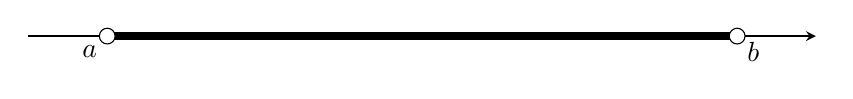
\begin{tikzpicture}[x=1cm,y=1cm]
            \draw[->,>=stealth,semithick] (-5,0)--(5,0)node[below]{$\RR$}; %x軸
            \draw[thick] (-2,0)--(2,0); %
            \fill[black!100] (-4,0.05) rectangle (4,-0.05);

            \draw[thick] (-4,-0.2) node[left]{\(a\)};
            \draw[thick] (4,-0.2) node[right]{\(b\)};
            
            \fill[black!0](4,0) ellipse (0.1 and 0.1);
            \draw (4,0) ellipse (0.1 and 0.1);

            \fill[black!0](-4,0) ellipse (0.1 and 0.1);
            \draw (-4,0) ellipse (0.1 and 0.1);

            %\draw[thick] (-3,0.1)--(-3,-0.1) node[below]{\(x\)};
        \end{tikzpicture}
        \caption{開区間は閉区間の開集合}
        \label{fig:loc-closed-closure}
    \end{figure}

    条件\eqref{lc-intersection}:    
    例えば\(\left]a,b\right[\)を直径とする
    開円盤\(U\)を
    \[
        U\coloneqq\left\{z\in\CC;\ 
        \left\lvert z-\frac{a+b}{2}\right\rvert 
        < \frac{b-a}{2}\right\}
    \]
    で定義し,閉集合\(F\)として閉区間\([a,b]\)をとれば,
    \({\left]a,b\right[}= U\cap F\)とかける.(図\ref{fig:loc-closed-intersection}参照)
    \begin{figure}[htb]
        \centering
        %\scalebox{0.8}{
            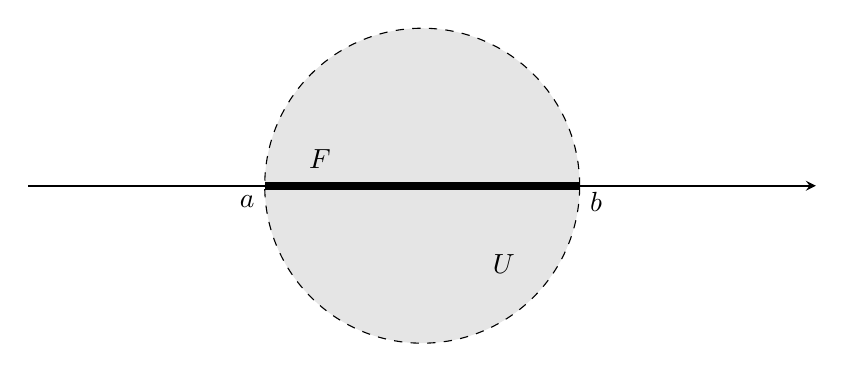
\begin{tikzpicture}[x=1cm]
            \fill[black!10] (0.7,0.1) (0,0) ellipse (2 and 2);
            \draw[dashed,black!100] (0.7,0.1) (0,0) ellipse (2 and 2);
            \draw[->,>=stealth,semithick] (-5,0)--(5,0)node[below]{$\RR$}; %x軸
            \draw[thick] (-2,0)--(2,0); %
            \fill[black!100] (-2,0.05) rectangle (2,-0.05);

            \draw[thick] (-2,-0.2) node[left]{\(a\)};
            \draw[thick] (2,-0.2) node[right]{\(b\)};
            \draw (-1.3,0.1) node[above]{$F$};
            \draw (1.3,-1) node[left]{$U$};

            %\fill[black!100](2,0) ellipse (0.1 and 0.1);
            %\draw (2,0) ellipse (0.1 and 0.1);

            %\fill[black!100](-2,0) ellipse (0.1 and 0.1);
            %\draw (-2,0) ellipse (0.1 and 0.1);
        \end{tikzpicture}%}
        \caption{開区間は円盤と閉区間の合併}
        \label{fig:loc-closed-intersection}
    \end{figure}

    条件\eqref{lc-neighbor}:実数\(a<x<b\)に対して,
    条件\eqref{lc-intersection}のときと同様に,
    \[
        U\coloneqq\left\{z\in\CC;\ 
        \left\lvert z-\frac{a+b}{2}\right\rvert 
        < \frac{b-a}{2}\right\}
    \]とすれば,\(U\)は\(x\)の開近傍で\({\left]a,b\right[}\cap U\)は\(U\)の閉集合となる.
    もう少し小さい近傍として,例えば\(x\)を中心とする開円盤
    \[
        U\coloneqq\left\{z\in\CC;
        \left\lvert z-x\right\rvert 
        < \min\left(x-a,b-x,1\right)\right\}
    \]をとることもできる.(図\ref{fig:loc-closed-neibor}参照)
    \begin{figure}[htb]
        \centering
        %\scalebox{0.8}{
            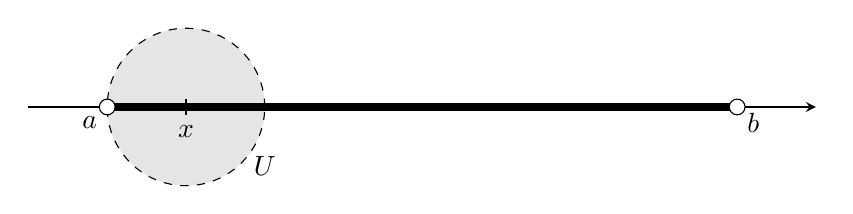
\begin{tikzpicture}[x=1cm,y=1cm]
            \fill[black!10] (-3,0) ellipse (1 and 1);
            \draw (-2,-0.5) node[below]{$U$};
            \draw[->,>=stealth,semithick] (-5,0)--(5,0)node[below]{$\RR$}; %x軸
            \draw[thick] (-2,0)--(2,0); %
            \fill[black!100] (-4,0.05) rectangle (4,-0.05);

            \draw[thick] (-4,-0.2) node[left]{\(a\)};
            \draw[thick] (4,-0.2) node[right]{\(b\)};

            \draw[dashed,black!100] (-3,0) ellipse (1 and 1);
            %\fill[black!0](-2,0) ellipse (0.1 and 0.1);
            %\draw (-2,0) ellipse (0.1 and 0.1);
            
            \fill[black!0](4,0) ellipse (0.1 and 0.1);
            \draw (4,0) ellipse (0.1 and 0.1);

            \fill[black!0](-4,0) ellipse (0.1 and 0.1);
            \draw (-4,0) ellipse (0.1 and 0.1);

            \draw[thick] (-3,0.1)--(-3,-0.1) node[below]{\(x\)};
        \end{tikzpicture}%}
        \caption{各点まわりで開区間と円盤の共通部分は円盤の閉集合}
        \label{fig:loc-closed-neibor}
    \end{figure}
\end{EG}























\section{局所コンパクト}

\begin{leftbar}
\begin{DFN}
    \(X\)をハウスドルフ空間とする.
    \begin{enumerate}
        \item \(X\)の部分集合\(A\subset X\)について,
        閉包\(\bar{A}\)がコンパクトであるとき,
        \(A\)は\textbf{相対コンパクト}であるという.
        \item 任意の点\(x\in X\)に対して,\(x\)の相対コンパクトな開近傍が存在するとき,
        \(X\)は\textbf{局所コンパクト空間}であるという.
    \end{enumerate}
\end{DFN}
\end{leftbar}

\begin{EG}
    位相多様体\(X\)は局所コンパクトである.
\end{EG}
\begin{proof}
    \(x\in X\)の近傍\(U_x\)でユークリッド空間の開集合\(U'_x\)と
    同相なものが存在する.\(U_x\)と\(U'_x\)の間の
    同相写像を\(\varphi\colon U_x\to U'_x\)とする.
    \(\varphi(x)\)を中心とする開球\(B_x\)で\(U'_x\)に含まれるものが存在する.
    この\(B_x\)に対し,\(\overline{B_x}\)はコンパクトである.
    したがって,\(\varphi^{-1}\left(\overline{B_x}\right)
    =\overline{\varphi^{-1}(B_x)}\)はコンパクトである.
    すなわち\(\varphi^{-1}(B_x)\)は\(x\)の相対コンパクトな開近傍である.
\end{proof}





次の命題から,局所コンパクト空間においては,部分集合が
局所コンパクトであることと局所閉であることは同じである.

\begin{PRP}
    \(X\)をハウスドルフ空間とする.
    \(X\)の部分空間\(A\)に関する次の条件
    \eqref{loc-cpt-subsp}と\eqref{loc-cpt-lc}
    について,一般に\eqref{loc-cpt-subsp}\(\Rightarrow\)\eqref{loc-cpt-lc}がなりたつ.
    \(X\)が局所コンパクトなら\eqref{loc-cpt-lc}\(\Rightarrow\)\eqref{loc-cpt-subsp}もなりたつ.
    \begin{enumerate}[(1)]%\setlength{\leftskip}{2zw}
        \item \(A\)は局所コンパクト空間である.\label{loc-cpt-subsp}
        \item \(A\)は\(X\)の局所閉集合である.\label{loc-cpt-lc}
    \end{enumerate}    
\end{PRP}

\subsection{局所コンパクトノルム空間の有限次元性}

有限次元ノルム空間\(X\)は局所コンパクト.
実際,実数\(r>0\)に対し,
開球\(D_r(0)\)は有界閉集合なのでコンパクトである.
したがって,
\(x\in X\)に対し,\(D_{\lVert x\rVert +1}(0)\)はコンパクト近傍である.

無限次元ノルム空間は局所コンパクトにはならない.\cite{Shw67}


\subsection{関数列の局所的な一様収束概念}
関数列の収束には各点収束と一様収束,その間の収束概念として広義一様収束があった.
関数列が定義される空間が局所コンパクトなら,
広義一様収束と局所一様収束の概念は一致する.
この辺はシュヴァルツ解析学1を参考にした.
金子関数論講義にも書いてある.
\begin{leftbar}
\begin{DFN}
    \(X\)を集合,\(Y\)を距離空間とする.
    \(
        \left(f_n\colon X\to Y\right)_{n\in \NN}
    \)
    を\(X\)から\(Y\)への写像の列とし,
    \(f\colon X\to Y\)を\(X\)から\(Y\)への写像とする.

    1.  
    列
    \(\left(f_n(x)\right)\)が\(X\)上で\(f(x)\)に
    \textbf{一様収束} (uniform conbergent) するとは,
    任意の実数\(q>0\)に対し,\(m\in\NN\)で
    \(n\geqq m\)をみたすすべての自然数\(n\)に対し\(X\)で
    \[
        \dist(f_n(x),f(x))<q
    \]
    をみたすものが存在することをいう.

    2. 
    \(X\)を位相空間とする.列
    \(\left(f_n\right)\)が\(X\)上で\(f\)に
    \textbf{広義一様収束}\footnotemark[1]するとは,
    \(X\)の任意のコンパクト集合\(K\)上で
    \(\left(f_n\right)\)が\(f\)に一様収束することをいう.

    3. 
    \(X\)を位相空間とする.
    列\(
        \left(f_n\colon X\to Y\right)_{n\in \NN}
    \)が\(X\)上で\(f\colon X\to Y\)に
    \textbf{局所一様} (locally uniform) に収束するとは,
    \(X\)の各点\(x\)に対して,
    \(x\)の開近傍\(U\in I_x\)で,
    \((f_n)\)が\(U\)上で\(n\to\infty\)で\(f\)に一様収束
    するものが存在することをいう.
\end{DFN}
\end{leftbar}
\footnotetext[1]{
        海外では,広義一様収束にあたる言葉はなく,
        いちいち,任意のコンパクト集合上で
        一様収束するというらしい.(金子)
        広義一様収束のことをコンパクト一様収束ということもある.
    }

    局所コンパクト空間\(X\)は各点がコンパクトな近傍を持つ.
\begin{PRP}
    \(X\)が局所コンパクト空間であるとする.\(Y\)を距離空間とする.
    このとき,列\(
        \left(f_n\colon X\to Y\right)_{n\in \NN}
    \)が\(X\)上で\(f\colon X\to Y\)に局所一様に収束することと,
    広義一様収束することは同値である.
\end{PRP}
\begin{proof}
    \(f_n\)が広義一様収束するとする.
    \(x\in X\)とする.
    \(X\)が局所コンパクトなので,
    \(x\)に対しコンパクトな近傍\(K\in I_x\)が存在する.
    この\(K\)に対し,
    \(f_n\)は\(K\)上一様収束する.
    よって,\(f_n\)は局所一様に収束する.

    \(f_n\)が局所一様に収束するとする.
    \(K\)を\(X\)のコンパクト集合とする.
    \(q>0\)を実数とする.
    各\(a\in K\)に対し,\(a\)の近傍\(U_a\in I_a\)で,
    \((f_n)\)が\(U_a\)上\(f\)に一様収束するものが存在する.
    この\(\left(U_a\right)_{a\in K}\)に対し,
    有限個の添え字を選んで,
    \(K\subset U_{a_1}\cup\dots\cup U_{a_n}\)とすることができる.
    \(m_i\)を\(n\geqq m_i\)となるすべての自然数\(n\)に対し,
    \(U_{a_i}\)上\[
        \dist(f_n(x),f(x))<q
    \]をみたすものとする.\(m=\max_i m_i\)とすると,
    \(n\geqq m\)となるすべての自然数\(n\)に対し,
    \(K\)上\[
        \dist(f_n(x),f(x))<q
    \]がなりたつ.
    よって,\(K\)上一様収束する.
\end{proof}


\subsection{無限遠点で可算な局所コンパクト空間}

\begin{leftbar}    
    \begin{DFN}
        \(X\)を局所コンパクト空間とする.\(X\)の1点コンパクト化を\(Y\)とし,
        \(b\in Y\)を無限遠点とする.
        \(X\)が\textbf{無限遠点で可算} (countable at infinity) である
        とは,\(b\)の近傍系で可算なものが存在することをいう.
    \end{DFN}
    \end{leftbar}
    


\begin{PRP}
    \(X\)を局所コンパクト空間とする.
    \(X\)が無限遠点で可算であることと,
    \(\sigma\)コンパクトであることは同値である.
\end{PRP}






















\section{パラコンパクト性}

\begin{DFN}[パラコンパクト]
    ハウスドルフ空間\(X\)がパラコンパクトであるとは,
    任意の開被覆が局所有限な細分をもつことをいう.
\end{DFN}

\begin{DFN}[第2可算]
    位相空間\(X\)が第2可算であるとは,
    開集合の基底で可算集合であるものが存在することをいう.
\end{DFN}

\begin{DFN}[\(\sigma\)コンパクト]
    位相空間\(X\)が\(\sigma\)コンパクトであるとは,
    コンパクト集合の列\((U_n)_{n\in\nn}\)で\(X\)の
    被覆であるものが存在することをいう.
\end{DFN}

\begin{PRP}
    位相多様体に対して次の条件(1)--(3)は同値である.
    \begin{enumerate}[(1)]
        \item 第2可算である.
        \item リンデレーフである.
        \item \(\sigma\)コンパクトである.
    \end{enumerate}
\end{PRP}




























%===============================================
% 参考文献スペース
%===============================================
\begin{thebibliography}{20} 
    \bibitem[Bou1]{Bou1} ブルバキ 位相1.
    \bibitem[Kan21]{Kan21} 金子晃, 関数論講義, サイエンス社, 2021.
    \bibitem[KS90]{KS90} Masaki Kashiwara, Pierre Schapira, 
        \textit{Sheaves on Manifolds}, 
        Grundlehren der Mathematischen Wissenschaften, 292, Springer, 1990.
    \bibitem[KS06]{KS06} Masaki Kashiwara, Pierre Schapira, 
        \textit{Categories and Sheaves}, 
        Grundlehren der Mathematischen Wissenschaften, 332, Springer, 2006.
    \bibitem[Mat65]{Mat65} 松島与三, 多様体入門, 裳華房, 1965.
    
    \bibitem[Mori81]{Mori81} 森田紀一, 位相空間論, 岩波書店, 1981.

    \bibitem[Sai09]{Sai09} 斎藤毅, 集合と位相, 東京大学出版会, 2009.
        
        第2可算,\(\sigma\)コンパクトの定義と,無限遠点で可算との同値性について.

    \bibitem[Shw67]{Shw67} シュヴァルツ解析学1, 東京図書, 1970.
    \bibitem[Sh16]{Sh16} 志甫淳, 層とホモロジー代数, 共立出版, 2016.
\end{thebibliography}

%===============================================


\end{document}
